\documentclass[aspectratio=169,10pt]{beamer}
\usepackage{graphicx}
\usepackage{booktabs}
\usepackage{array}
\usepackage{amsmath}
\usepackage{tikz}
\usetikzlibrary{arrows.meta,positioning}
\graphicspath{{../figures/}}

%,- red colour theme (as analysis_slides.tex),-
\definecolor{ubred}{RGB}{160,20,20}
\definecolor{ubdark}{RGB}{90,10,10}
\definecolor{ublight}{RGB}{205,70,70}
\usetheme{default}
\usecolortheme{default}
\setbeamercolor{structure}{fg=ubred}
\setbeamercolor{title}{fg=ubdark}
\setbeamercolor{frametitle}{fg=white,bg=ubred}
\setbeamercolor{section in head/foot}{fg=white,bg=ubdark}
\setbeamercolor{alerted text}{fg=ubred}
\setbeamercolor{block title}{fg=white,bg=ubred}
\setbeamercolor{block body}{bg=ubred!8}
\setbeamercolor{itemize item}{fg=ubred}
\setbeamercolor{itemize subitem}{fg=ublight}
\setbeamertemplate{navigation symbols}{}
\setbeamertemplate{frametitle}{\vskip4pt\usebeamercolor[fg]{frametitle}%
  \begin{beamercolorbox}[wd=\paperwidth,ht=2.4ex,dp=1ex,leftskip=.3cm]{frametitle}%
  \bfseries\insertframetitle\end{beamercolorbox}}
\newif\ifbackup
\setbeamertemplate{footline}{%
  \leavevmode\hbox{%
  \begin{beamercolorbox}[wd=.62\paperwidth,ht=2.4ex,dp=1ex,leftskip=.3cm]{section in head/foot}%
  \usebeamerfont{author in head/foot}\insertshortauthor\ | MicroBooNE NuMI CC$2\pi^{\pm}$\hfill\end{beamercolorbox}%
  \begin{beamercolorbox}[wd=.38\paperwidth,ht=2.4ex,dp=1ex,rightskip=.3cm]{section in head/foot}%
  \hfill\insertshorttitle\quad\ifbackup Backup \insertframenumber\else\insertframenumber\,/\,\pageref{mainend}\fi\end{beamercolorbox}}}

% figure with a placeholder while it does not exist
\newcommand{\fig}[2]{\IfFileExists{../figures/multipion/#1.pdf}{\includegraphics[width=#2]{multipion/#1}}%
  {\fbox{\parbox[c][3cm]{#2}{\centering\color{gray}figure \texttt{\detokenize{#1}}}}}}
\newcommand{\GeVc}{\,\text{GeV}/c}
\newcommand{\pot}{\,\text{POT}}

\title[CC$2\pi^{\pm}$ in NuMI]{$\nu_\mu+\bar\nu_\mu$ charged-current production of two charged pions on argon in the NuMI beam}
\subtitle{Selection, background constraint and extraction of the one-bin total (blind, pseudo-data)}
\author[Nowak et al.]{T.~Mahmud, L.~Gu, I.~Pophale, J.~Nowak}
\institute{Lancaster University}
\date{MicroBooNE cross-section group meeting, October 2026}

\begin{document}

{\setbeamertemplate{footline}{}
\begin{frame}[plain]
  \titlepage
  \begin{center}\small\color{ubdark}
  CC$2\pi^\pm Xp$ \;$\bullet$\; FHC, RHC, combined \;$\bullet$\; technical note draft 0.6
  \end{center}
\end{frame}}

\begin{frame}{Outline}
  \begin{columns}[T]
  \column{.48\textwidth}
  \textbf{\color{ubred}Introduction}
  \begin{enumerate}\small
    \item Why two charged pions
    \item Starting point and history
    \item What is reused from the BNB CC$2\pi^\pm Np$ analysis
    \item Signal definition, samples, blindness
  \end{enumerate}
  \vspace{2mm}
  \textbf{\color{ubred}Selection}
  \begin{enumerate}\small\setcounter{enumi}{4}
    \item Particle classifier
    \item Track assignment and event classifier
    \item Working point and the detector term
  \end{enumerate}
  \column{.48\textwidth}
  \textbf{\color{ubred}Extraction and validation}
  \begin{enumerate}\small\setcounter{enumi}{7}
    \item Sidebands and the background constraint
    \item Extraction through the framework
    \item Beam-on data in the control regions
    \item Ensembles and selection variants
    \item Measurements of variables
    \item Three or more pions
  \end{enumerate}
  \vspace{2mm}
  \textbf{\color{ubred}To do and conclusions}\\[1mm]
  \textbf{\color{ubred}Backup}
  \end{columns}
\end{frame}

% ===================== INTRODUCTION =====================
\section{Introduction}

\begin{frame}{Why two charged pions}
  \begin{columns}[T]
  \column{.56\textwidth}
  \begin{itemize}\small\setlength\itemsep{3pt}
    \item CC multi-pion production sits at the transition between resonant production (higher $N^*$
          and $\Delta$ states) and shallow and deep inelastic scattering, where models differ most.
    \item The observed charged-pion multiplicity is shaped by the intranuclear cascade: pions are
          absorbed, charge-exchanged or produced in re-scattering before they leave the nucleus, so a
          two-pion final state probes FSI directly.
    \item Multi-pion events are a background of the single-pion and pion-less measurements (a lost or
          misidentified pion); a measured rate on argon constrains the model used across the programme.
    \item NuMI at MicroBooNE: higher-energy tail than the BNB and $35$--$55\%$ $\bar\nu_\mu$, so it
          complements the BNB CC$2\pi^\pm Np$ analysis.
  \end{itemize}
  \column{.42\textwidth}
  \begin{block}{\small Goal of this stage}\small
    \begin{itemize}\setlength\itemsep{2pt}
      \item A selection of $\nu_\mu+\bar\nu_\mu$ CC$2\pi^\pm Xp$ on the full NuMI exposure
      \item The one-bin total in FHC, RHC and combined, through the extraction framework, with a
            background constraint
      \item Validation on pseudo-data and checks of the inputs with beam-on data in the opened control
            regions
      \item Then the differential observables
    \end{itemize}
  \end{block}
  \vspace{1mm}
  {\footnotesize The two-pion signal region is blind; every result shown is extracted from pseudo-data.}
  \end{columns}
\end{frame}

\begin{frame}{Starting point and history}
  \begin{itemize}\footnotesize\setlength\itemsep{1pt}
    \item Built on the NuMI CC$1\pi^\pm$ analysis (Pophale, Nowak; release v1.9): samples, per-run POT
          normalisation, beam-off and dirt, systematic universes, detector variations, Wiener-SVD
          unfolding, MCS calibration of exiting tracks.
    \item First draft (2026-08-13; T.~Mahmud, L.~Gu): \texttt{CC1mu2pi}, \texttt{CC1mu3pi} as sub-selections of
          the single-pion selection with a looser pion BDT, Run-1 FHC overlay only. On the full exposure:
          $18.2\%$ efficiency, $26\%$ purity, expected total uncertainty $89\%$.
    \item Rebuilt since on the strategy of the BNB CC$2\pi^\pm Np$ analysis (N.~Majeed, internal note v2,
          May 2026) and on the current single-pion release.
  \end{itemize}
  \begin{center}\fig{unc_evolution}{0.64\textwidth}\end{center}
  \vspace{-3mm}
  {\scriptsize Expected total uncertainty of the combined one-bin total along the analysis (the first four from the
  study outside the framework, without constraint).}
\end{frame}

\begin{frame}{Reused from the BNB CC$2\pi^\pm Np$ analysis}
  \scriptsize\renewcommand{\arraystretch}{1.05}
  \begin{tabular}{>{\raggedright\arraybackslash}p{0.36\textwidth}>{\raggedright\arraybackslash}p{0.58\textwidth}}
    \toprule
    Element (BNB note) & In the NuMI analysis \\
    \midrule
    Two-stage identification: per-track classifiers, best-assignment hypothesis, then an event
    classifier (BNB: purity $1\%\to44\%$) &
    Adopted. The event classifier is where the purity comes from. \\
    Assignment by the largest product of particle scores &
    Adopted: largest summed log-probability over all choices of one muon and $N$ pions (at most eight
    tracks); best and runner-up for $N=1,2,3$. \\
    Event features: assigned scores, per-type sums, counts above threshold &
    Adopted, plus $L_2-L_1$, $L_2-L_3$, runner-up margin, track and shower counts, topological score,
    CosmicIP (33 features). \\
    Background categories by topology &
    Adopted (CC$1\pi$, CC$\geq3\pi$, CC$\pi^0$, CC$0\pi$, NC, out of FV, dirt, beam-off). \\
    Sidebands from the classifier outputs, each aimed at one migration path (1$\mu$3$\pi$, 1$\mu$3p,
    BDT band) &
    Adopted: three-pion-like, proton-like, score band, low score. \\
    Conditional-covariance constraint (\texttt{ConstrainedCalculator}); BNB: $27.3\%\to21.5\%$, not applied &
    Adopted after alternative-model closure: the lever on the $(1+B/S)$ amplification of the flux. \\
    One-bin total first, differential second; Recomb2 leads the detector term &
    Same order; Recomb2 also leads here. \\
    \bottomrule
  \end{tabular}
\end{frame}

\begin{frame}{Adapted for NuMI, and what is not reused}
  \begin{columns}[T]
  \column{.58\textwidth}
  \textbf{\color{ubred}Adapted}
  \begin{itemize}\footnotesize\setlength\itemsep{2pt}
    \item \textbf{Particle ID}: one four-class XGBoost ($\mu,\pi,p$, other) instead of three binary
          classifiers; ``other'' = tracks without a truth match (cosmics). No NuGraph inputs (not in
          the NuMI ntuples). Deployed on LLR score and geometry only, for robustness against the
          detector variations.
    \item \textbf{Training}: no signal-enhanced NuMI samples; all 14 overlays. Particle classifier:
          whole run periods held out. Event classifier: two-fold by event parity, on the nominal mixture
          (overlay, dirt, beam-off, CV weights); the BNB meta-BDT saw enhanced samples only.
    \item \textbf{Signal}: $\nu_\mu+\bar\nu_\mu$, $p_\mu>0.15$, every $p_\pi>0.10\GeVc$, $\pi^0$/kaon veto,
          any number of protons (BNB: $\nu_\mu$, KE $>10$ MeV, $\geq1p$). The $\geq1p$ subsample ($81\%$)
          is kept for comparison.
    \item \textbf{Working point}: on the expected total uncertainty of the one-bin total, not on
          efficiency $\times$ purity.
    \item \textbf{Containment}: not required (BNB: all $\pi$ and $p$ contained, a third of the efficiency).
  \end{itemize}
  \column{.40\textwidth}
  \textbf{\color{ubred}Not reused}
  \begin{itemize}\footnotesize\setlength\itemsep{2pt}
    \item KE $>10$ MeV thresholds: that phase space is mostly not reconstructed.
    \item Invariant masses as results: the reco pion energy saturates, so the masses are squeezed
          towards threshold; study products unless a binning passes the $0.50$ criterion.
  \end{itemize}
  \vspace{2mm}
  \textbf{\color{ubred}Comparison}\\[1mm]
  \scriptsize\setlength{\tabcolsep}{3pt}
  \begin{tabular}{lcc}
    \toprule
    & BNB & NuMI (comb.) \\
    \midrule
    Efficiency & $4$--$6\%$ & $15\%$ \\
    Purity & $47$--$58\%$ & $48\%$ \\
    Detector, predicted count$^*$ & $11.0\%$ & $8.4\%$ \\
    Total, constrained & $21.5\%^\dagger$ & $16.5\%$ \\
    \bottomrule
  \end{tabular}\\[0.5mm]
  {\tiny $^*$the seven BNB variations; $^\dagger$evaluated, not applied in the BNB note}
  \end{columns}
\end{frame}

\begin{frame}{Signal definition and scope}
  \begin{block}{\small Signal: CC$2\pi^\pm Xp$}\small
    $\nu_\mu$ or $\bar\nu_\mu$ CC, vertex in the fiducial volume of the single-pion analysis, one muon with
    $p_\mu>0.15\GeVc$, exactly two charged pions leaving the nucleus, both with $p_\pi>0.10\GeVc$ (a
    third charged pion at any momentum makes the event background); no $\pi^0$, kaon or heavier meson;
    any number of nucleons; $\theta(\mu,\text{leading }\pi)<2.6$ rad.
  \end{block}
  \begin{columns}[T]
  \column{.50\textwidth}
  \begin{itemize}\footnotesize\setlength\itemsep{2pt}
    \item Leading = hardest pion (truth). Pion charge not measured.
    \item $0.10\GeVc$ is the pion tracking turn-on: it removes the unreconstructable $10\%$ and keeps
          $90\%$ of the two-pion signal. Efficiency is limited by reconstructing several tracks from one
          vertex, not by the soft pions.
    \item Events with a third charged pion below $0.10\GeVc$ amount to $6.2\%$ of the signal (Run-4 FHC
          overlay) and are background by definition.
    \item Subsample with $\geq1$ proton above $0.3\GeVc$: $81\%$.
  \end{itemize}
  \column{.48\textwidth}
  \scriptsize
  \begin{tabular}{lp{0.82\textwidth}}
    \toprule
    D1 & Inclusive in nucleons, with a $\geq1p$ subsample \\
    D2 & $p_\pi>0.10\GeVc$; pion-momentum bins only above $0.175\GeVc$ \\
    D3 & The two-pion signal region is blind \\
    D4 & NuGraph inputs: deferred (not available for NuMI) \\
    D5 & NuMI NuWro overlay: only if it can be validated \\
    D6 & Reco counterpart of the $2.6$ rad opening-angle cut \\
    D7 & No exclusivity cut against the blind single-pion signal region \\
    D8 & Measurements stop at two pions; $\geq3\pi$ is a control sample \\
    \bottomrule
  \end{tabular}
  \end{columns}
\end{frame}

\begin{frame}{Samples, exposure and blindness}
  \begin{itemize}\small\setlength\itemsep{3pt}
    \item Samples and normalisation of the single-pion release: 14 $\nu_\mu$ overlays (FHC Runs 1, 2, 4, 5;
          RHC Runs 1, 2, 3, 4a, 4b, 4c), 7 beam-off, 7 dirt samples, each run normalised to its own exposure.
    \item Exposure: $7.766\times10^{20}\pot$ FHC, $1.1082\times10^{21}\pot$ RHC, $1.8848\times10^{21}\pot$ combined.
    \item Detector variations: Run-4 FHC and RHC, CV + eight variations (LY down, LY Rayleigh,
          Recomb2, SCE, wire modification $x$, $yz$, angle $xz$, angle $yz$).
    \item Systematics: PPFX flux universes, GENIE multisim and unisims, Geant4 reinteraction, POT,
          targets, simulation statistics; detector variations taken fractionally (DVfrac).
    \item Pseudo-data: Poisson throws, run by run, of overlays and dirt at the data exposure; the
          framework adds the beam-off.
    \item Beam-on data used only in the opened control regions of the single-pion analysis, with both
          signal regions removed.
  \end{itemize}
  \vspace{2mm}
  \begin{center}
  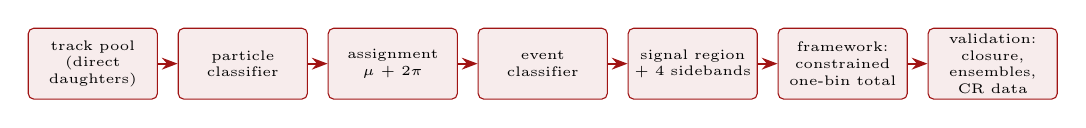
\begin{tikzpicture}[node distance=2.5mm, every node/.style={font=\tiny, align=center},
      box/.style={draw=ubred, fill=ubred!8, rounded corners=2pt, minimum height=9mm, text width=15mm, inner sep=2pt},
      arr/.style={-{Stealth[length=2mm]}, ubred, thick}]
    \node[box] (a) {track pool\\(direct daughters)};
    \node[box, right=of a] (b) {particle\\classifier};
    \node[box, right=of b] (c) {assignment\\$\mu+2\pi$};
    \node[box, right=of c] (d) {event\\classifier};
    \node[box, right=of d] (e) {signal region\\+ 4 sidebands};
    \node[box, right=of e] (f) {framework:\\constrained\\one-bin total};
    \node[box, right=of f] (g) {validation:\\closure, ensembles,\\CR data};
    \draw[arr] (a)--(b); \draw[arr] (b)--(c); \draw[arr] (c)--(d); \draw[arr] (d)--(e);
    \draw[arr] (e)--(f); \draw[arr] (f)--(g);
  \end{tikzpicture}
  \end{center}
\end{frame}

% ===================== SELECTION =====================
\section{Selection}

\begin{frame}{Starting point: the cut-based selection}
  \begin{columns}[T]
  \column{.52\textwidth}
  \scriptsize\setlength{\tabcolsep}{3pt}
  \begin{tabular}{lrrrcc}
    \toprule
    & Gen.\ sig. & Sel.\ sig. & Sel.\ total & Eff. & Purity \\
    \midrule
    $2\pi$ FHC  & $1\,210$ & $221$ & $836$    & $18.2\%$ & $26.4\%$ \\
    $2\pi$ RHC  & $1\,672$ & $303$ & $1\,168$ & $18.1\%$ & $26.0\%$ \\
    $2\pi$ comb.& $2\,882$ & $524$ & $2\,004$ & $18.2\%$ & $26.1\%$ \\
    \midrule
    $3\pi$ comb.& $551$ & $54.5$ & $517$ & $9.9\%$ & $10.5\%$ \\
    \bottomrule
  \end{tabular}
  \vspace{2mm}
  \begin{itemize}\footnotesize\setlength\itemsep{2pt}
    \item \texttt{CC1mu1piXp} preselection with a looser pion ID (vertex distance $\leq9.5$ cm, the
          first-draft pion BDT, up to two uncontained candidates), $\theta(\mu,\text{longest }\pi)<2.6$ rad.
    \item Backgrounds: CC$1\pi$ with a second candidate $22\%$, CC$\pi^0$ $21\%$, CC$\geq3\pi$ $7\%$,
          NC $6\%$, beam-off $2.5\%$.
    \item Both candidates are true pions in only $60\%$ of the selected signal.
  \end{itemize}
  \column{.46\textwidth}
  \begin{block}{\small Why purity is the lever}\footnotesize
    The flux uncertainty ($\approx17\%$) scales signal and background together, so after background
    subtraction it enters the extracted total as
    \[ \delta_\text{flux}\approx17\%\times(1+B/S). \]
    At $26\%$ purity: flux $65\%$, cross section $47\%$, detector $34\%$, total $89\%$.
  \end{block}
  \vspace{1mm}
  {\footnotesize Two ways out: raise $S/B$ (classifiers), and constrain $B$ with control samples that share
  its composition (sidebands).}
  \end{columns}
\end{frame}

\begin{frame}{Particle classifier}
  \begin{columns}[T]
  \column{.50\textwidth}
  \begin{itemize}\footnotesize\setlength\itemsep{2pt}
    \item XGBoost, four classes ($\mu$, $\pi$, $p$, other) on the tracks of the pion-candidate pool
          (generation 2, track score $\geq0.3$) of all 14 overlays: $3.1$M tracks.
    \item Labels from the backtracked particle; tracks without a truth match (mostly overlay cosmics)
          are ``other''.
    \item Training: Runs 1, 2, 4 of both horn modes; held out: RHC Run 3, FHC Run 5.
    \item The Run 1--3 beam-on, beam-off and dirt ntuples lack 20 track branches, so the deployed
          models use the 43 inputs every sample carries.
    \item Evaluated in the selection through ROOT \texttt{RBDT}, identical to XGBoost.
  \end{itemize}
  \vspace{1mm}
  \scriptsize\setlength{\tabcolsep}{3pt}
  \begin{tabular}{lccc}
    \toprule
    Pion identification (63 inputs) & $\pi$/rest & $\pi$/$p$ & $\pi$/$\mu$ \\
    \midrule
    Particle classifier         & $0.954$ & $0.985$ & $0.895$ \\
    First-draft pion BDT        & $0.888$ & $0.945$ & $0.804$ \\
    Single-pion pion BDT        & $0.818$ & $0.961$ & $0.558$ \\
    LLR score                   & $0.670$ & $0.893$ & $0.251$ \\
    \bottomrule
  \end{tabular}\\[0.5mm]
  {\tiny Table: held-out tracks with a truth match. Figure: the whole pool of the held-out runs, unmatched tracks
  as ``other''.}
  \column{.48\textwidth}
  \centering\fig{pid_roc}{\textwidth}\\[1mm]
  \begin{itemize}\footnotesize\setlength\itemsep{1pt}
    \item At the first-draft pion efficiency ($91.8\%$): candidate purity $27.6\%\to43.3\%$, protons
          passing $13.4\%\to4.1\%$.
    \item Same gain in FHC and RHC, for $\pi^+$ and $\pi^-$. Muon vs pion is the hardest separation.
  \end{itemize}
  \end{columns}
\end{frame}

\begin{frame}{The LLR-and-geometry particle classifier}
  \begin{columns}[T]
  \column{.50\textwidth}
  \begin{itemize}\footnotesize\setlength\itemsep{3pt}
    \item The detector variations move the calorimetric inputs ($\chi^2$ scores, PIDA, Bragg
          likelihoods, calorimetric energies) by up to half their spread for protons; the LLR score by
          at most $0.04$; geometric inputs not at all.
    \item The deployed classifier keeps only: LLR score (sum and per plane), length, track score, vertex
          distance, start and end containment, range and MCS momenta, proton-hypothesis energy,
          daughter counts, per-plane hit flags.
    \item Pion ROC area $0.892$ vs $0.926$ for the 43-input model over all held-out tracks ($0.903$ vs $0.938$
          on the pool); at $80\%$ pion efficiency $9.0\%$ of protons pass (vs $3.9\%$).
    \item It halves the part of the detector term that no constraint can reach (efficiency part
          $14.3\%\to7.8\%$; next slides).
  \end{itemize}
  \column{.48\textwidth}
  \centering\fig{pid_probs}{\textwidth}\\
  {\scriptsize $P(\pi)$ of the deployed classifier by true class, held-out runs.}
  \end{columns}
\end{frame}

\begin{frame}{Track assignment}
  \begin{itemize}\small\setlength\itemsep{3pt}
    \item Events with one neutrino slice and the vertex in the FV; tracks of the pool with track score
          $\geq0.5$, the muon candidate included, carry the four class probabilities.
    \item Hypothesis ``one muon, $N$ pions, the rest protons or other'':
    \[ L_N=\log P_\mu(\mu)+\sum_{\text{pions}}\log P_\pi+\sum_{\text{rest}}\log\left(1-P_\mu-P_\pi\right) \]
          probabilities floored at $10^{-6}$; every choice among at most eight tracks enumerated (ranked by
          $\max(P_\mu,P_\pi)$); best and runner-up kept for $N=1,2,3$.
    \item In the selected signal (held-out runs): the assigned muon is a true muon in $89\%$, each assigned
          pion a true charged pion in $88\%$, all three in $76\%$.
    \item In the preselected signal only $30\%$ of events have the muon and both pions reconstructed as
          tracks, so in most signal events no assignment can be fully right: the event classifier has to
          work with partial topologies.
    \item Every track gets a role: second pion and proton candidates become available for observables,
          categories and the response.
  \end{itemize}
\end{frame}

\begin{frame}{Event classifier}
  \begin{columns}[T]
  \column{.48\textwidth}
  \begin{itemize}\footnotesize\setlength\itemsep{2pt}
    \item XGBoost, two-pion signal vs everything else, 33 features: probabilities of the assigned tracks,
          $L_2-L_1$, $L_2-L_3$, margin over the runner-up, class sums and counts above $0.5$, track and
          shower counts, topological score, CosmicIP.
    \item Domain: one slice, vertex in FV, software trigger, $\geq3$ tracks,
          $\theta(\mu,\text{longer assigned }\pi)<2.6$ rad.
    \item Trained on Runs 1, 2, 4 ($206$k events, $13.6$k signal) with the nominal mixture of overlay,
          dirt and beam-off and CV weights; tested on FHC Run 5 and RHC Run 3 ($105$k, $7.3$k signal).
          The test periods also choose the working point (validation periods).
    \item ROC area $0.887$. Kinematic features of the assigned tracks give $0.898$, a gain that disappears
          in the total uncertainty: not used.
    \item Largest gains: summed $P(\pi)$, $L_2$, number of tracks with $P_\pi>0.5$, topological score,
          number with $P_\mu>0.5$.
  \end{itemize}
  \column{.50\textwidth}
  \centering\fig{evt_score}{\textwidth}\\
  {\scriptsize Event score, test periods projected to the full exposure (combined).}
  \end{columns}
\end{frame}

\begin{frame}{Working point: minimum of the expected total uncertainty}
  \begin{columns}[T]
  \column{.58\textwidth}
  \centering\fig{wp_scan}{\textwidth}
  \column{.40\textwidth}
  \begin{itemize}\footnotesize\setlength\itemsep{2pt}
    \item Threshold chosen on the expected total of the one-bin total with all terms: data statistics,
          flux, POT and targets, cross section, reinteraction, detector (eight Run-4 variations, FHC and RHC
          correlated), simulation statistics.
    \item Statistics and flux alone would push to $3.9\%$ efficiency; the detector term rises steeply above
          $0.95$. Minimum at $0.92$, flat from $0.90$ to $0.94$.
  \end{itemize}
  \vspace{1mm}
  \scriptsize\setlength{\tabcolsep}{2.5pt}
  \begin{tabular}{lccc}
    \toprule
    Selection & Eff. & Pur. & Total \\
    \midrule
    Cut-based \texttt{CC1mu2pi}   & $18.2\%$ & $26\%$ & $89\%$ \\
    + particle classifier         & $15.8\%$ & $35\%$ & $61\%$ \\
    Event cl., 43 inputs          & $17.1\%$ & $56\%$ & $47\%$ \\
    Event cl., LLR and geometry   & $13.0\%$ & $51\%$ & $46\%$ \\
    \bottomrule
  \end{tabular}\\[1mm]
  {\scriptsize Combined configuration, no constraint, score $>0.92$. Flux $17\%\times(1+B/S)$, except the last row
  (PPFX universes, as in the constraint study); the scan gives $44\%$ at $0.92$ with the proxy.}
  \end{columns}
\end{frame}

\begin{frame}{Selection requirements of \texttt{CC1mu2piBDT}}
  \footnotesize
  \begin{columns}[T]
  \column{.56\textwidth}
  \setlength{\tabcolsep}{3pt}
  \begin{tabular}{rlp{0.62\textwidth}}
    \toprule
    & Cut & Requirement \\
    \midrule
    1 & Slices & exactly one neutrino slice \\
    2 & Vertex & in the single-pion FV, outside the dead-wire region in $z$ \\
    3 & Trigger & software trigger passed \\
    4 & Track score & $\geq0.5$ (direct neutrino daughters) \\
    5 & PID inputs & LLR in $(-1,2)$; $p$, $\mu$, MIP Bragg in $(0,500)$; length $>0$ \\
    6 & Ranking & by $\max(P_\mu,P_\pi)$; at most eight tracks \\
    7 & Pool size & at least three tracks \\
    8 & Assignment & muon and two pions maximising $L_2$ \\
    9 & Opening angle & $\theta(\mu,\text{longer assigned }\pi)<2.6$ rad \\
    10 & Event score & $>0.90$ (two-fold classifier): signal region \\
    \bottomrule
  \end{tabular}
  \column{.42\textwidth}
  \begin{itemize}\footnotesize\setlength\itemsep{3pt}
    \item Cuts 1--9 define the domain of the event classifier; cut 10 the signal region.
    \item Cut 5 is a validity requirement of the pool (the Bragg likelihoods exist in every run; they are
          not classifier inputs).
    \item The single-pion cuts after its preselection (topological score $>0.67$, muon, containment,
          wire-gap, shower and multiplicity cuts) are not applied; topological score, CosmicIP, track and
          shower counts enter only as features.
    \item Sidebands: cuts 1--9 and score $\leq0.90$ (next section).
  \end{itemize}
  \end{columns}
\end{frame}

\begin{frame}{The detector term}
  \begin{columns}[T]
  \column{.50\textwidth}
  \begin{itemize}\footnotesize\setlength\itemsep{2pt}
    \item With the 43-input classifier the detector term ($33\%$) is the largest. A paired bootstrap
          (one Poisson weight per physical event, shared by CV and variations) attributes $7.7\%$ of it to
          the statistics of the variation samples.
    \item Sources: Recomb2 ($+22\%$), wire modification angle $yz$ ($+18\%$), $x$ ($+12\%$), $yz$
          ($+8\%$); LY, SCE and angle $xz$ consistent with zero.
    \item The variations lower the selected signal by $\approx8\%$ and the background by
          $10$--$18\%$: an efficiency part, which no background constraint removes, and a background part.
    \item Training on the variation samples did not help. The LLR-and-geometry classifier halves the
          efficiency part and is adopted.
    \item In the BNB convention (predicted selected count): $10.6\%$ (8 variations), $8.4\%$ (the BNB seven),
          against $11.0\%$ in the BNB note. The extracted total amplifies it by $2$--$4$.
  \end{itemize}
  \column{.48\textwidth}
  \scriptsize\setlength{\tabcolsep}{2.5pt}
  \begin{tabular}{llcccc}
    \toprule
    Particle cl. & Features & Pur. & Detector & (eff., bkg.) & Total \\
    \midrule
    43 inputs & PID set  & $56\%$ & $32.7\%$ & ($14.3$, $17.8$) & $47\%$ \\
    43 inputs & full set & $62\%$ & $33.0\%$ & ($18.2$, $14.8$) & $45\%$ \\
    no $\chi^2$/PIDA/$E$ & PID set & $57\%$ & $35.1\%$ & ($14.9$, $19.0$) & $48\%$ \\
    LLR+geom. & PID set  & $51\%$ & $21.4\%$ & ($7.8$, $15.2$) & $44\%$ \\
    LLR+geom. & full set & $55\%$ & $20.3\%$ & ($8.4$, $12.9$) & $42\%$ \\
    \bottomrule
  \end{tabular}\\[1mm]
  {\scriptsize Combined configuration, best threshold of each, no constraint. Totals within the $3\%$ scatter of
  the scans.}
  \end{columns}
\end{frame}

% ===================== CONSTRAINT =====================
\section{Constraint}

\begin{frame}{Signal region and sidebands}
  \begin{columns}[T]
  \column{.50\textwidth}
  \begin{itemize}\footnotesize\setlength\itemsep{2pt}
    \item Four sidebands from the classifier outputs, exclusive, assigned in this order inside the
          two-pion domain (cuts 1--9, score $\leq0.90$):
    \begin{itemize}\footnotesize
      \item three-pion-like: $\geq4$ tracks and $L_3>L_2$ (the $\geq3\pi$ control sample, D8; BNB 1$\mu$3$\pi$)
      \item proton-like: an assigned pion with $P_p>0.5$ (BNB 1$\mu$3p)
      \item score band $0.5$--$0.90$
      \item low score $<0.5$
    \end{itemize}
    \item The sidebands leave out the events of the blind single-pion signal region, so they can be
          opened without it.
    \item Of the signal-region events $14\%$ lie in the blind single-pion signal region (kept, D7) and $12\%$
          in its opened multi-$\pi$ control region.
  \end{itemize}
  \column{.48\textwidth}
  \centering\fig{region_composition}{0.88\textwidth}\\
  {\scriptsize Predicted composition (single classifier), combined, full exposure; table: two-fold, all periods.}\\[1mm]
  \scriptsize\setlength{\tabcolsep}{3pt}
  \begin{tabular}{lrrc}
    \toprule
    Region & Events & Signal & Purity \\
    \midrule
    Signal region & $920$ & $444$ & $48\%$ \\
    Three-pion-like & $294$ & $36$ & $12\%$ \\
    Proton-like & $16\,640$ & $458$ & $3\%$ \\
    Score $0.5$--$0.90$ & $4\,534$ & $655$ & $14\%$ \\
    Score $<0.5$ & $13\,162$ & $166$ & $1\%$ \\
    \bottomrule
  \end{tabular}

  \end{columns}
\end{frame}

\begin{frame}{Background constraint: conditional covariance}
  \begin{columns}[T]
  \column{.52\textwidth}
  \begin{itemize}\footnotesize\setlength\itemsep{2pt}
    \item Covariance of the predicted counts in the signal region ($s$) and the sidebands ($c$), built
          from every source, conditioned on the sideband data $d_c$:
    \[ \hat n_s=n_s+V_{sc}V_{cc}^{-1}(d_c-n_c),\qquad V'_{ss}=V_{ss}-V_{sc}V_{cc}^{-1}V_{cs} \]
          (\texttt{ConstrainedCalculator}, the tool of the BNB note).
    \item The flux scales the background and the sidebands alike: flux $38\%\to5.0\%$. Detector
          $23.5\%\to9.3\%$, close to its efficiency part.
    \item Three-pion-like alone ($294$ events) halves the total. Data statistics grow, since the sideband
          counts enter the background estimate.
  \end{itemize}
  \vspace{1mm}
  \scriptsize\setlength{\tabcolsep}{2.5pt}
  \begin{tabular}{lccccc}
    \toprule
    Constraint & Total & Flux & Xsec & Det. & Data st. \\
    \midrule
    None & $50.1\%$ & $38.2\%$ & $19.4\%$ & $23.5\%$ & $6.9\%$ \\
    Three-pion-like & $27.8\%$ & $15.3\%$ & $9.5\%$ & $15.5\%$ & $11.9\%$ \\
    Proton-like & $34.9\%$ & $13.3\%$ & $15.9\%$ & $26.3\%$ & $7.1\%$ \\
    Score $0.5$--$0.90$ & $22.1\%$ & $5.1\%$ & $8.2\%$ & $17.3\%$ & $7.6\%$ \\
    Score $<0.5$ & $35.5\%$ & $13.4\%$ & $10.9\%$ & $29.2\%$ & $7.5\%$ \\
    All sidebands & $16.5\%$ & $5.0\%$ & $6.7\%$ & $9.3\%$ & $8.6\%$ \\
    \bottomrule
  \end{tabular}
  \column{.46\textwidth}
  \centering\fig{region_corr}{0.92\textwidth}\\
  {\scriptsize Correlation of the predicted region counts under the systematic covariance (combined).
  Study outside the framework.}
  \end{columns}
\end{frame}

\begin{frame}{Closure under alternative models and the signal in the sidebands}
  \begin{columns}[T]
  \column{.50\textwidth}
  \textbf{\color{ubred}Alternative-model closure}
  \begin{itemize}\footnotesize\setlength\itemsep{2pt}
    \item Pseudo-data from a reweighted model in every region, extracted with the nominal model:
    \begin{itemize}\footnotesize
      \item GENIE multisim universe 545: $0.965$ ($-0.21\sigma$) constrained, $0.988$ without
      \item $\Delta\to N\pi$ angular: $0.995$ ($-0.03\sigma$), $1.014$ without
    \end{itemize}
    \item Over all GENIE multisim universes: bias rms $4.0\%$ with the constraint, every universe within
          $1\sigma$; $20.3\%$ without.
    \item These models lie inside the covariance: the test checks the procedure, not the model space.
  \end{itemize}
  \column{.48\textwidth}
  \textbf{\color{ubred}Signal in the sidebands}
  \begin{itemize}\footnotesize\setlength\itemsep{2pt}
    \item The score band holds more predicted signal than the signal region ($655$ vs $444$). Signal
          variations move every region together, so the conditioning also carries the signal model from the
          sidebands into the signal region.
    \item Nominal (framework): the signal covariance between regions is kept, since the same flux and interaction
          parameters act coherently on one CC$2\pi$ process in every region. The decorrelated variants are
          conservative stress tests:
  \end{itemize}
  \scriptsize\setlength{\tabcolsep}{3pt}
  \begin{tabular}{lc}
    \toprule
    Variant (study) & Constrained total \\
    \midrule
    Nominal & $16.5\%$ \\
    Sideband signal decoupled & $19.6\%$ \\
    Without the score band & $21.2\%$ \\
    Both & $23.9\%$ \\
    \bottomrule
  \end{tabular}\\[1mm]
  {\scriptsize Every variant closes within $0.25\sigma$ for both models. Score-band/SR signal ratio (single model): $1.684$
  nominal, $1.660$ (u545), $1.681$ ($\Delta\to N\pi$): these models do not probe the transfer; the stress model
  of the ensembles slides does.}
  \end{columns}
\end{frame}

% ===================== FRAMEWORK =====================
\section{Framework}

\begin{frame}{Extraction through the framework}
  \begin{columns}[T]
  \column{.52\textwidth}
  \begin{itemize}\footnotesize\setlength\itemsep{2pt}
    \item \texttt{CC1mu2piBDT} in the selection framework: track pool, class probabilities (\texttt{RBDT}),
          assignment, 33 features, event score, region.
    \item On a $30$k-event slice: features identical to the Python study, scores to $6\times10^{-8}$,
          regions in every event; \texttt{CC1mu1piXp} bitwise unchanged.
    \item 28 release samples and 18 detector-variation samples processed.
    \item Bin configuration: signal region as an ordinary bin, the four sidebands as sideband bins in the
          signal block (their signal is predicted).
    \item \texttt{Calculator Constrained} in the extraction configuration; the terms by source add up to the
          constrained total.
  \end{itemize}
  \column{.46\textwidth}
  \begin{block}{\small Detector-variation normalisation}\footnotesize
    Per POT the Run-4 detVar CV samples predict $1.27$ (FHC) and $1.51$ (RHC) times the nominal rate:
    they were simulated with the earlier NuMI flux. The absolute detector covariance carried that ratio.
    \begin{itemize}\footnotesize
      \item \texttt{DVfrac}: fractional change of each variation applied to the nominal prediction
            (also in the single-pion release since v1.8).
      \item Variation samples weighted to the current flux (per-event weight branch).
    \end{itemize}
    Constrained combined total: $17.9\%$ (absolute) $\to15.7\%$ (fractional, with or without the flux weight).
  \end{block}
  \end{columns}
\end{frame}

\begin{frame}{Overtraining found: the two-fold event classifier}
  \begin{columns}[T]
  \column{.52\textwidth}
  \begin{itemize}\footnotesize\setlength\itemsep{2pt}
    \item Efficiency in the classifier training periods $14.04\pm0.21\%$, validation periods $13.16\pm0.31\%$ ($2.4\sigma$).
    \item Cause: the event classifier was trained on a random $80\%$ of the training-period events. At score $>0.92$,
          within the domain:
  \end{itemize}
  \scriptsize\setlength{\tabcolsep}{3pt}
  \begin{tabular}{lcc}
    \toprule
    Events & Efficiency & Purity \\
    \midrule
    its training events (80\%) & $23.61\pm0.36\%$ & $55.4\%$ \\
    held-out 20\%, same periods & $21.35\pm0.71\%$ & $51.0\%$ \\
    validation periods & $21.18\pm0.48\%$ & $51.4\%$ \\
    \bottomrule
  \end{tabular}
  \begin{itemize}\footnotesize\setlength\itemsep{2pt}
    \item On data: efficiency $\approx+6\%$, background $\approx-4\%$, about $-2\%$ on the total; invisible to closure and
          ensembles (their pseudo-data are the same events).
  \end{itemize}
  \column{.46\textwidth}
  \begin{block}{\small Fix: two folds by event number}\footnotesize
    \begin{itemize}\setlength\itemsep{2pt}
      \item Models trained on even and on odd event numbers; every event, data included, scored by the model of the
            other parity. C++ $=$ Python to $6\times10^{-8}$.
      \item Working point rescanned (study, constrained comb.): $17.4/20.4/16.5/19.5/25.5\%$ at
            $0.85/0.88/0.90/0.92/0.94$ $\Rightarrow$ $0.90$.
      \item Signal region $920$ events, $444$ signal, purity $48\%$, efficiency $15\%$.
      \item All 46 samples reprocessed; total, variables and ensembles re-extracted (next slides).
    \end{itemize}
  \end{block}
  \end{columns}
\end{frame}

\begin{frame}{One-bin total: uncertainties (two-fold classifier, working point 0.90)}
  \begin{center}\fig{unc_breakdown}{0.72\textwidth}\end{center}
  \vspace{-2mm}
  \begin{columns}[T]
  \column{.52\textwidth}
  \scriptsize\setlength{\tabcolsep}{2.5pt}
  \begin{tabular}{lcccc}
    \toprule
    & Total & Data stat. & Detector & Unf./truth \\
    \midrule
    FHC, constrained & $21.5\%$ & $13.9\%$ & $10.9\%$ & $1.068$ \\
    RHC, constrained & $20.0\%$ & $11.0\%$ & $14.4\%$ & $1.059$ \\
    Comb., none      & $49.9\%$ & $6.5\%$  & $29.3\%$ & $1.093$ \\
    Comb., constrained & $16.5\%$ & $8.9\%$ & $10.2\%$ & $1.059$ \\
    \bottomrule
  \end{tabular}
  \column{.46\textwidth}
  \begin{itemize}\scriptsize\setlength\itemsep{1pt}
    \item With the constraint, data statistics are the largest term.
    \item Single model: $15.2\%$ (combined).
    \item MCS-calibration term, two-fold: $5.9/5.9/4.7\%$ (FHC/RHC/comb.), $0.29$ of the total.
    \item Unfolded/truth: one realisation; ensemble means within $1\%$.
    \item With it and the soft-pion term (next slides): $23.8/22.4/19.0\%$ constrained.
  \end{itemize}
  \end{columns}
\end{frame}

% ===================== CR DATA =====================
\section{Control-region data}

\begin{frame}{Beam-on data in the control regions: MCS momentum}
  \begin{columns}[T]
  \column{.46\textwidth}
  \begin{itemize}\footnotesize\setlength\itemsep{2pt}
    \item Inputs and output of the selection compared with beam-on data in the four opened control regions
          of the single-pion analysis; events of both signal regions removed. Shape tests per run period,
          summed.
    \item In the two-pion domain data/prediction $1.10$--$1.24$, as outside it ($1.12$).
    \item MCS momentum of the pool tracks: data/prediction $1.14$ at $0.7$--$0.9\GeVc$, $0.39$ at
          $1.8$--$1.9\GeVc$, $\chi^2=2234/19$.
    \item The exiting-track effect of the single-pion analysis (angular noise at the MCS segment scale).
          Its v1.9 calibration map (cells of $|\cos\theta_x|$ and length) applied to the classifier inputs of
          every simulated exiting track: $\chi^2=71.5/19$; $P(\mu)$ $1100\to293$, $P(\pi)$ $256\to56$.
  \end{itemize}
  \column{.52\textwidth}
  \centering\fig{cr_mcs}{\textwidth}
  \end{columns}
\end{frame}

\begin{frame}{Beam-on data in the control regions: LLR of long protons}
  \begin{columns}[T]
  \column{.46\textwidth}
  \begin{itemize}\footnotesize\setlength\itemsep{2pt}
    \item Pool tracks longer than $40$ cm with LLR $<-0.9$: $11\times$ more frequent in data ($592$ vs $52$).
    \item Long contained protons: both ends contained ($97\%$), from the vertex, $40$--$100$ cm, true
          protons in $72\%$ of the predicted; every period, both productions, all planes.
    \item Same hit count, more proton-like per hit in data: median LLR sum $-436$ to $-486$ (Run 4 data)
          vs $-339$ (simulation).
    \item Recomb2 reproduces it (median $-445$; share beyond $-0.9$: $0.15$ vs $0.16$--$0.23$ data,
          $0.015$ CV); the wire-response variations move it the other way.
    \item The classifier still calls them protons: $P_p>0.5$ for $86$--$92\%$ in every LLR band, data and
          simulation within $1$--$2\%$.
    \item Recomb2 strength fitted with all other terms: $1.44\pm0.50$; results move by $\leq0.40\sigma$,
          $\leq0.12\sigma$ beyond the Recomb2 term.
  \end{itemize}
  \column{.52\textwidth}
  \centering\fig{cr_llr}{\textwidth}
  \end{columns}
\end{frame}

\begin{frame}{Control regions: event score and summed $P(\pi)$}
  \begin{columns}[T]
  \column{.49\textwidth}
  \centering\fig{cr_score_2f}{\textwidth}
  \column{.49\textwidth}
  \centering\fig{cr_ppi}{\textwidth}
  \end{columns}
  \vspace{1mm}
  \begin{itemize}\footnotesize\setlength\itemsep{1pt}
    \item Two-pion domain of the control regions (signal regions removed); prediction normalised to the data
          ($\times1.14$); band: full systematic covariance of the shape.
    \item Event score with statistics only: $\chi^2=140/22$ after the calibration ($160/22$ before); the bin below the
          cut holds $0.83$ of the predicted share, Recomb2 gives $0.86$.
  \end{itemize}
\end{frame}

\begin{frame}{Control regions: shape tests with the systematic covariance}
  \begin{columns}[T]
  \column{.46\textwidth}
  \begin{itemize}\footnotesize\setlength\itemsep{3pt}
    \item Covariance of the prediction: flux, cross-section and reinteraction universes, the eight detector
          variations taken fractionally per horn mode (with the statistics of the variation samples), simulation
          and data statistics.
    \item Prediction normalised to the data total; the last non-empty bin dropped for the inversion, so
          ndf = non-empty bins $-1$; least-squares solve.
    \item Event score, class probabilities and MCS momentum are statistically compatible with the data under the
          full prediction covariance.
    \item The LLR score of the pool tracks remains incompatible with the data ($p=0.014$) at its proton end, where
          the long protons sit; the detector term alone takes it from $398$ to $36$.
  \end{itemize}
  \column{.52\textwidth}
  \scriptsize\setlength{\tabcolsep}{3pt}
  \begin{tabular}{lccc}
    \toprule
    Quantity & Stat.\ only & Full covariance & $p$ \\
    \midrule
    Event score & $98.5/11$ & $6.5/11$ & $0.84$ \\
    Event score, two-fold & $80.8/11$ & $7.4/11$ & $0.76$ \\
    Summed $P(\pi)$ & $23.6/7$ & $2.0/7$ & $0.96$ \\
    Track $P(\mu)$ & $48.1/9$ & $4.2/9$ & $0.90$ \\
    Track $P(\pi)$ & $40.4/9$ & $4.2/9$ & $0.90$ \\
    MCS momentum & $65.2/8$ & $6.2/8$ & $0.63$ \\
    LLR score & $397.8/9$ & $20.8/9$ & $0.014$ \\
    \bottomrule
  \end{tabular}\\[1mm]
  {\scriptsize Same, coarser bins in both columns (the statistics-only values of the previous slides use finer bins).}
  \end{columns}
\end{frame}

\begin{frame}{MCS calibration in the extraction}
  \begin{itemize}\small\setlength\itemsep{3pt}
    \item Overlays, dirt and detector-variation samples reprocessed with the calibrated classifier inputs;
          pseudo-data thrown with the same seeds (same events).
    \item Expected signal-region content changes by less than $1\%$ (signal $-0.9\%$ FHC, $-0.5\%$ RHC);
          constrained combined total $15.7\%\to15.2\%$.
    \item About $5\%$ of the signal-region events migrate in or out; their pseudo-data counts are independent
          Poisson draws, which moves the single-realisation closure to $1.05$--$1.09$
          ($+0.9\sigma$ FHC, $+2.3\sigma$ RHC of the migrating events' Poisson spread).
    \item Calibration uncertainty as in the single-pion analysis: pseudo-data calibrated with each of the seven
          alternative maps, extracted with the nominal response, four fully correlated terms.
    \begin{itemize}\small
      \item $2.2\%$ of the constrained combined total, $2.3$--$5.5\%$ elsewhere, at most $0.24$ of the total
            (two-fold classifier: $4.7\%$, $0.29$; shifts within $3.1\times$ their noise).
      \item Each map moves $4$--$19$ events; every shift within $1.7\times$ their Poisson noise: an upper estimate.
    \end{itemize}
    \item The calibrated selection is used from here on.
  \end{itemize}
\end{frame}

% ===================== VALIDATION =====================
\section{Validation}

\begin{frame}{Ensembles of pseudo-experiments}
  \begin{columns}[T]
  \column{.50\textwidth}
  \begin{itemize}\footnotesize\setlength\itemsep{2pt}
    \item Members thrown from the simulation (eight per-run files each), each extracted through the framework with
          and without the constraint; seed of each file a hash of (ensemble, member, file).
    \item Two-fold classifier, 200 members: offset $+0.0$ to $+1.0\%$ ($\pm0.5$--$0.8\%$), FHC, RHC, combined.
    \item Without the constraint: pull width $0.96$--$1.01$, $70$--$72\%$ inside the $68\%$ interval, as expected.
    \item With the constraint: width $0.81$--$0.85$ ($76$--$78\%$ inside): the quoted term propagates the data with the
          gain of the whole prediction (signal included), the estimator with the background gain: $8.6\%$ vs $7.6\%$
          (ratio $0.88$); with the fixed beam-off ($0.98$) the measured width.
    \item The first ensemble (100 members, consecutive seeds) had width $0.85$ also without the constraint: an
          artefact of the seeding, gone with hashed seeds.
  \end{itemize}
  \column{.48\textwidth}
  \centering\fig{ens_pulls_2f}{0.94\textwidth}\\
  {\scriptsize Pulls of the two-fold ensemble, combined configuration, without and with the constraint.}
  \end{columns}
\end{frame}

\begin{frame}{Ensembles under alternative and stress models}
  \begin{columns}[T]
  \column{.42\textwidth}
  \begin{itemize}\scriptsize\setlength\itemsep{2pt}
    \item 50 members each, nominal response; combined, constrained (single model $\to$ two-fold):
  \end{itemize}
  \scriptsize\setlength{\tabcolsep}{2pt}
  \begin{tabular}{lcc}
    \toprule
    Model & single & two-fold \\
    \midrule
    GENIE u545, $\Delta\to N\pi$ & $\leq0.17\sigma$ & $\leq0.11\sigma$ \\
    score-band signal $+20\%$ & $-0.54\sigma$ & $-0.47\sigma$ \\
    $\geq3\pi$ $+30\%$, $1\pi$ $-20\%$ & $+0.04\sigma$ & \\
    signal $\times(1+0.5\sin p_\pi^{\rm lead})$ & $-0.24\sigma$ & \\
    signal $\times(1+0.5\cos\pi p_\pi^{\rm soft}/0.5)$ & $-0.44\sigma$ & $-0.32\sigma$ \\
    \bottomrule
  \end{tabular}
  \begin{itemize}\scriptsize\setlength\itemsep{2pt}
    \item Signal changes carried by the sidebands pull the constrained result towards the model; the soft-pion
          change is an efficiency effect (same bias without the constraint).
    \item Without the score band (framework, same members): total $20.4\%$ (vs $15.9\%$), score-band stress
          $-0.30\sigma$, softest-pion unchanged.
  \end{itemize}
  \column{.56\textwidth}
  \centering\fig{ens_altmodels_2f}{\textwidth}\\
  {\scriptsize Two-fold classifier: reweighted and stress models.}
  \end{columns}
\end{frame}

\begin{frame}{Soft pions: covariance against generators}
  \begin{itemize}\footnotesize\setlength\itemsep{2pt}
    \item Efficiency $4\%$ at $p_\pi^{\rm soft}=0.10$--$0.125\GeVc$, $14\%$ at $0.15$--$0.175$, $17$--$21\%$ up to $0.6\GeVc$, $15\%$ above.
    \item 600 GENIE universes: $30$--$40\%$ of the signal below $0.175\GeVc$ (CV $35\%$); efficiency through the
          spectrum $\pm1.2\%$. Stress model: $46\%$, $-7.4\%$ ($3.8\sigma$ of the universes).
    \item Standalone generators, reweighted against GENIE: NuWro $35\%$ / $+1.8\%$, NEUT $44\%$ / $-4.4\%$, GiBUU
          $52\%$ / $-8.3\%$. The stress model is inside the generator range, outside the covariance.
    \item A $0.175\GeVc$ cut does not help (the softer events stay as background); migration across $0.10\GeVc$ $<1\%$.
    \item Added: soft-pion efficiency term = generator envelope, $8.5/8.1/8.3\%$ (FHC/RHC/comb.), $4$--$12\%$ per
          differential bin.
  \end{itemize}
  \centering\fig{softpion}{0.95\textwidth}
\end{frame}

\begin{frame}{Selection variants}
  \begin{itemize}\small\setlength\itemsep{3pt}
    \item Working point rescanned on the constrained combined total (score $0.85$--$0.96$, study): $0.92$
          remains the minimum ($16.8\%$; $15.2\%$ through the framework). Tighter thresholds reach
          $58$--$70\%$ purity at $22$--$32\%$ total.
    \item Per horn mode: FHC minimum at $0.90$ ($25.9\%$; $27.3\%$ at $0.92$, within $2.7$ points from
          $0.85$ to $0.95$); RHC at $0.92$ ($19.3\%$). One threshold kept.
    \item Shower features (energy, vertex distance, track score and direction of the leading shower; with
          dE/dx, second shower and two-shower mass in a larger set): ROC area $0.874\to0.884$--$0.887$,
          purity $+2$ points at fixed threshold.
    \begin{itemize}\small
      \item In the $\pi^0$ control region the leading-shower energy, distance, score and direction follow the
            data; its dE/dx and the multi-shower features do not ($\chi^2$ $22$--$63$ for $3$--$6$ dof).
    \end{itemize}
    \item Best constrained totals of the variants (with and without shower features, calorimetric particle
          classifier): $16.3$--$17.3\%$ ($21.1\%$ calorimetric without showers) vs $16.8\%$ adopted. The
          detector term of one variant moves by $3$--$6$ points between neighbouring thresholds, more than
          these differences.
    \item The selection is kept.
  \end{itemize}
\end{frame}

% ===================== VARIABLES =====================
\section{Variables}

\begin{frame}{Measurements of variables: definitions and status}
  \begin{columns}[T]
  \column{.56\textwidth}
  \scriptsize\setlength{\tabcolsep}{3pt}
  \begin{tabular}{lp{0.70\textwidth}}
    \toprule
    Variable & Reco (assigned tracks) / truth \\
    \midrule
    $p_\mu$ & range if the end is contained, else MCS (v1.9 calibration for simulated tracks) / true $p_\mu$ \\
    $\cos\theta_\mu$ & about the target-to-vertex direction / about the true $\nu$ direction \\
    $\cos\theta_\pi^{\rm fwd}$, $\cos\theta_\pi^{\rm bwd}$ & the more forward and the more backward pion \\
    $\cos\theta_{\pi\pi}$ & opening angle of the two pions \\
    $\cos\theta_{\mu\pi}$ & muon and the closer pion \\
    $p_\pi^{\rm low}$, $p_\pi^{\rm high}$ & range momentum, both pions contained (pion mass from equal $T/m$) \\
    $N_p$ & unassigned track with $P_p>0.5$ / proton above $0.3\GeVc$ \\
    \bottomrule
  \end{tabular}\\[1mm]
  {\tiny The pions are ordered by the variable itself, the same way at truth and reco level, so the convention is
  symmetric in the two pions.}
  \column{.42\textwidth}
  \begin{itemize}\footnotesize\setlength\itemsep{3pt}
    \item Binning: contiguous bins with $P(\text{reco bin }i\,|\,\text{true bin }i)\geq0.50$ (the criterion of the
          single-pion release) and at least 40 predicted signal events per bin.
    \item Combined, full exposure, two-fold classifier: signal region $920$ events, $444$ signal (all periods).
    \item $\sqrt{N}/S$: data statistics of the background-subtracted bin, before unfolding and constraint.
    \item Selection branches for these variables (equal to this study to $10^{-7}$, all other branches unchanged);
          46 samples reprocessed; univmake and the Wiener-SVD extraction per variable, with and without the
          constraint (results after the feasibility slides).
  \end{itemize}
  \end{columns}
\end{frame}

\begin{frame}{Muon momentum and angle}
  \begin{columns}[T]
  \column{.78\textwidth}
  \centering\fig{kin2f_pmu}{\textwidth}\\[-1mm]
  \fig{kin2f_cmu}{\textwidth}
  \column{.21\textwidth}
  \begin{itemize}\scriptsize\setlength\itemsep{2pt}
    \item $p_\mu$: 5 bins, $P(r|t)$ $0.50$--$0.68$, $P(t|r)$ $0.30$--$0.95$, $\sqrt{N}/S$ $12$--$20\%$; MCS sets the resolution above $0.65\GeVc$.
    \item $\cos\theta_\mu$: 6 bins, $P(r|t)$ $0.73$--$0.91$, $13$--$23\%$; forward-peaked, the last bin $0.95$--$1$.
    \item Efficiency rises with $p_\mu$ and forward angle ($10.5\%\to15\%$).
  \end{itemize}
  \end{columns}
\end{frame}

\begin{frame}{Pion angles}
  \begin{columns}[T]
  \column{.78\textwidth}
  \centering\fig{kin2f_cfwd}{\textwidth}\\[-1mm]
  \fig{kin2f_cbwd}{\textwidth}
  \column{.21\textwidth}
  \begin{itemize}\scriptsize\setlength\itemsep{2pt}
    \item Forward pion: 6 bins, $P(r|t)$ $0.61$--$0.78$.
    \item Backward pion: 8 bins over the full range, $P(r|t)$ $0.64$--$0.83$.
    \item $\sqrt{N}/S$ $13$--$22\%$; efficiency flat ($11$--$15\%$).
    \item Angles are the best-measured pion quantities: the direction does not depend on the pion stopping.
  \end{itemize}
  \end{columns}
\end{frame}

\begin{frame}{Opening angles}
  \begin{columns}[T]
  \column{.78\textwidth}
  \centering\fig{kin2f_cpipi}{\textwidth}\\[-1mm]
  \fig{kin2f_cmupi}{\textwidth}
  \column{.21\textwidth}
  \begin{itemize}\scriptsize\setlength\itemsep{2pt}
    \item $\cos\theta_{\pi\pi}$: 8 bins, $P(r|t)$ $0.53$--$0.71$; sensitive to the resonance decay and to FSI.
    \item $\cos\theta_{\mu\pi}$ (closer pion): 7 bins, $P(r|t)$ $0.53$--$0.79$.
    \item $\sqrt{N}/S$ $14$--$22\%$ per bin.
  \end{itemize}
  \end{columns}
\end{frame}

\begin{frame}{Pion momenta}
  \begin{columns}[T]
  \column{.78\textwidth}
  \centering\fig{kin2f_ppi_lo}{\textwidth}\\[-1mm]
  \fig{kin2f_ppi_hi}{\textwidth}
  \column{.21\textwidth}
  \begin{itemize}\scriptsize\setlength\itemsep{2pt}
    \item Both assigned pions contained in $79\%$ of the selected signal, but the range momentum saturates
          (pions interact before stopping): only 3 ($p_\pi^{\rm low}$) and 2 ($p_\pi^{\rm high}$) bins pass.
    \item D2 allows pion-momentum bins only above $0.175\GeVc$: $p_\pi^{\rm low}$ would keep 2 bins.
    \item Low information; candidates for a coarse result only.
  \end{itemize}
  \end{columns}
\end{frame}

\begin{frame}{Proton multiplicity and summary}
  \begin{columns}[T]
  \column{.52\textwidth}
  \centering\fig{kin2f_np}{\textwidth}\\
  {\scriptsize $N_p$: 0 and $\geq1$ protons above $0.3\GeVc$; $P(r|t)$ $0.92$ and $0.73$, $P(t|r)$ $0.36$ and $0.98$;
  $\sqrt{N}/S$ $12\%$ and $8\%$.
  The $\geq1p$ bin is the comparison with the BNB CC$2\pi^\pm Np$ result.}
  \column{.46\textwidth}
  \scriptsize\setlength{\tabcolsep}{3pt}
  \begin{tabular}{lcccc}
    \toprule
    Variable & Bins & $P(r|t)$ & $P(t|r)$ & $\sqrt{N}/S$ \\
    \midrule
    $p_\mu$ & 5 & $0.50$--$0.68$ & $0.30$--$0.95$ & $12$--$20\%$ \\
    $\cos\theta_\mu$ & 6 & $0.73$--$0.91$ & $0.72$--$0.82$ & $13$--$23\%$ \\
    $\cos\theta_\pi^{\rm fwd}$ & 6 & $0.61$--$0.78$ & $0.56$--$0.82$ & $13$--$20\%$ \\
    $\cos\theta_\pi^{\rm bwd}$ & 8 & $0.64$--$0.83$ & $0.62$--$0.83$ & $16$--$22\%$ \\
    $\cos\theta_{\pi\pi}$ & 8 & $0.53$--$0.71$ & $0.53$--$0.82$ & $16$--$22\%$ \\
    $\cos\theta_{\mu\pi}$ & 7 & $0.53$--$0.79$ & $0.49$--$0.77$ & $14$--$21\%$ \\
    $p_\pi^{\rm low}$ & 3 & $0.56$--$0.63$ & $0.35$--$0.84$ & $13$--$15\%$ \\
    $p_\pi^{\rm high}$ & 2 & $0.74$--$0.75$ & $0.30$--$0.95$ & $9$--$14\%$ \\
    $N_p$ & 2 & $0.73$--$0.92$ & $0.36$--$0.98$ & $8$--$12\%$ \\
    \bottomrule
  \end{tabular}\\[1mm]
  {\scriptsize Two-fold classifier. $P(t|r)$: reconstructed-bin purity of the signal; lowest where neighbouring true
  bins feed in, corrected by the unfolding.}
  \end{columns}
\end{frame}

\begin{frame}{Differential extraction through the framework}
  \begin{columns}[T]
  \column{.62\textwidth}
  \centering\fig{kin2f_results_comb}{\textwidth}\\
  {\scriptsize Two-fold classifier, combined, sideband constraint: unfolded pseudo-data, $A_C$-smeared truth and tune.}
  \column{.36\textwidth}
  \scriptsize\setlength{\tabcolsep}{2pt}
  \begin{tabular}{lccc}
    \toprule
    & \multicolumn{2}{c}{Per bin} & $\chi^2$ \\
    Variable & none & constr. & truth \\
    \midrule
    $p_\mu$ & $45$--$60\%$ & $17$--$32\%$ & $0.2/5$ \\
    $\cos\theta_\mu$ & $40$--$123\%$ & $17$--$54\%$ & $0.8/6$ \\
    $\cos\theta_\pi^{\rm fwd}$ & $51$--$113\%$ & $22$--$52\%$ & $1.9/6$ \\
    $\cos\theta_\pi^{\rm bwd}$ & $45$--$99\%$ & $15$--$42\%$ & $0.6/8$ \\
    $\cos\theta_{\pi\pi}$ & $43$--$66\%$ & $17$--$32\%$ & $1.0/8$ \\
    $\cos\theta_{\mu\pi}$ & $40$--$185\%$ & $18$--$45\%$ & $4.1/7$ \\
    $N_p$ & $44$--$130\%$ & $20$--$58\%$ & $0.1/2$ \\
    \bottomrule
  \end{tabular}
  \begin{itemize}\scriptsize\setlength\itemsep{1pt}
    \item Wiener-SVD (filter on), FHC, RHC, combined; all 42 compatible with their truth in the nominal realisation.
    \item The constraint is essential: it halves the per-bin uncertainty or better.
    \item Integrals (full covariance) $15$--$18\%$, as the one-bin total; bin averages $21$--$39\%$.
  \end{itemize}
  \end{columns}
\end{frame}

\begin{frame}{Three or more pions}
  \begin{columns}[T]
  \column{.55\textwidth}
  \begin{itemize}\footnotesize\setlength\itemsep{3pt}
    \item In the two-pion domain, events with $\geq4$ tracks and $L_3>L_2$: $234$ at full exposure
          (combined, 43-input classifier), of which $88$ have $\geq3$ charged pions, $41$ a $\pi^0$, $35$
          are two-pion signal.
    \item A three-pion event classifier built the same way: ROC area $0.855$, but every three-pion selection
          has a total uncertainty above $100\%$ (\texttt{CC1mu3pi} $245\%$, with the particle classifier
          $117\%$, event classifier at best $105\%$).
    \item Four and five pions: $3.1$ selected four-pion signal events at $4.8\%$ purity and $0.1$ five-pion.
    \item $P(\text{reco bin}\,|\,\text{true bin})$ of the pion multiplicity: $0.84$, $0.48$, $0.33$ for
          $1$, $2$, $\geq3$ pions.
  \end{itemize}
  \column{.43\textwidth}
  \begin{block}{\small D8}\footnotesize
    The measurements stop at two pions. The three-pion-like events are a sideband of the two-pion
    constraint, as the 1$\mu$3$\pi$ sideband of the BNB note; alone it halves the total uncertainty.
  \end{block}
  \end{columns}
\end{frame}

% ===================== TODO & CONCLUSIONS =====================
\section{Summary}

\begin{frame}{To do}
  \begin{columns}[T]
  \column{.50\textwidth}
  \textbf{\color{ubred}Before unblinding the one-bin total}
  \begin{itemize}\footnotesize\setlength\itemsep{2pt}
    \item Decide between the nominal constraint ($16.5\%$) and the reduced-transfer one without the score band
          (framework: $20.4\%$, half the signal-model transfer).
    \item Two-pion signal region opened only after the single-pion one (D7).
  \end{itemize}
  \column{.48\textwidth}
  \textbf{\color{ubred}Towards the cross sections}
  \begin{itemize}\footnotesize\setlength\itemsep{2pt}
    \item Generator predictions with the two-pion signal definition (GENIE tunes, NuWro, NEUT, GiBUU).
    \item Differential variables: extracted, compatible with their truth in the nominal pseudo-data; next ensembles and alternative models per
          variable, generator predictions. Invariant masses stay study products unless they pass the $0.50$ criterion.
    \item The $\geq1p$ subsample for the comparison with the BNB result.
    \item Independent-generator closure if a NuMI NuWro overlay can be validated (D5); NuGraph inputs if
          NuMI samples appear (D4).
    \item The same sideband constraint for the single-pion analysis, on pseudo-data.
  \end{itemize}
  \end{columns}
\end{frame}

\begin{frame}{Conclusions}
  \begin{itemize}\footnotesize\setlength\itemsep{3pt}
    \item A $\nu_\mu+\bar\nu_\mu$ CC$2\pi^\pm Xp$ selection on the full NuMI exposure
          ($1.88\times10^{21}\pot$), built on the two-stage strategy of the BNB CC$2\pi^\pm Np$ analysis and
          adapted to NuMI: four-class particle classifier on LLR and geometry, best assignment, event
          classifier in two folds by event number (no overtraining). Combined: $15\%$ efficiency, $48\%$ purity, $920$ predicted events ($444$ signal).
    \item Without a constraint the one-bin total carries $50\%$, dominated by the flux amplified by the
          background subtraction and by the detector variations. Four classifier-defined sidebands bring it
          to $16.5\%$ combined ($21.5\%$ FHC, $20.0\%$ RHC) through the framework; data statistics are then
          the largest term. With the MCS-calibration ($4.7\%$) and soft-pion ($8.3\%$) terms: $19.0\%$.
    \item Fixed for both analyses on the way: the detector-variation samples carry the earlier NuMI flux.
    \item Validation on pseudo-data: ensembles return the expected truth within $1\%$, with nominal coverage
          without the constraint and a conservative statistical term with it; alternative models close within
          $0.11\sigma$; a score-band signal stress moves the constrained total by $-0.47\sigma$.
    \item Differential variables: $p_\mu$, $\cos\theta_\mu$, the two pion angles, the opening angles and the proton
          multiplicity pass the $0.50$ criterion with 2 to 8 bins at $8$--$23\%$ data statistics per bin; the
          pion momenta give only 2 or 3 bins. Through the framework all seven are compatible with their truth in the
          nominal pseudo-data, $15$--$58\%$ per bin (combined, constrained).
    \item Beam-on control regions: with the single-pion MCS calibration, the classifier inputs and the event score
          are compatible with the data under the full prediction covariance; the LLR score at its proton end (long protons) follows the
          recombination variation at $1.4$ times its size ($\leq0.12\sigma$ beyond the detector term).
    \item Three or more pions are not measurable at this exposure and serve as a control sample.
  \end{itemize}
  \label{mainend}
\end{frame}

% ===================== BACKUP =====================
\backuptrue
\appendix
\section*{Backup}

{\setbeamertemplate{footline}{}
\begin{frame}[plain]
  \begin{center}\Huge\color{ubred} Backup\end{center}
\end{frame}}

\begin{frame}{Backup: detector-variation treatments}
  \small
  \begin{center}\setlength{\tabcolsep}{4pt}
  \begin{tabular}{lcccccc}
    \toprule
    & \multicolumn{2}{c}{Absolute} & \multicolumn{2}{c}{Fractional} & \multicolumn{2}{c}{Fractional, flux-weighted} \\
    \cmidrule(lr){2-3}\cmidrule(lr){4-5}\cmidrule(lr){6-7}
    & Detector & Total & Detector & Total & Detector & Total \\
    \midrule
    FHC, no constraint       & $40.8\%$ & $58.4\%$ & $29.8\%$ & $51.3\%$ & $34.2\%$ & $54.0\%$ \\
    FHC, constrained         & $15.4\%$ & $24.9\%$ & $11.9\%$ & $22.4\%$ & $11.4\%$ & $22.5\%$ \\
    RHC, no constraint       & $28.4\%$ & $46.6\%$ & $17.9\%$ & $41.0\%$ & $18.1\%$ & $41.1\%$ \\
    RHC, constrained         & $11.1\%$ & $18.5\%$ & $7.6\%$  & $16.3\%$ & $7.3\%$  & $16.3\%$ \\
    Combined, no constraint  & $33.4\%$ & $50.7\%$ & $23.0\%$ & $44.5\%$ & $25.9\%$ & $46.0\%$ \\
    Combined, constrained    & $11.9\%$ & $17.9\%$ & $8.5\%$  & $15.7\%$ & $8.2\%$  & $15.7\%$ \\
    \bottomrule
  \end{tabular}
  \end{center}
  \begin{itemize}\footnotesize\setlength\itemsep{2pt}
    \item Weighted to the current flux the detVar CV predicts $0.94$ of the nominal rate, flat in energy; the
          origin of that offset is not identified, and the fractional treatment cancels it.
    \item The ratio variation/CV changes by at most $0.027$ (median $0.003$) with the flux weight; above
          $1$ GeV it follows the integral within the variation-sample statistics ($5$--$6\%$).
    \item Before the MCS calibration (the calibrated totals are on the uncertainty slide).
  \end{itemize}
\end{frame}

\begin{frame}{Backup: framework totals before and after the MCS calibration}
  \footnotesize
  \begin{center}\setlength{\tabcolsep}{3.5pt}
  \begin{tabular}{llcccccc}
    \toprule
    & & Total & Detector & Flux & Cross sect. & Data stat. & Unf./truth \\
    \midrule
    FHC & none        & $54.0\to51.3$ & $34.2\to30.9$ & $37.0\to36.2$ & $14.7\to14.6$ & $10.5\to10.4$ & $1.056\to1.082$ \\
    FHC & constrained & $22.5\to21.3$ & $11.4\to10.6$ & $6.1\to6.2$   & $8.7\to7.8$   & $14.0\to13.5$ & $1.020\to1.050$ \\
    RHC & none        & $41.1\to40.3$ & $18.1\to19.3$ & $31.5\to30.1$ & $15.5\to15.0$ & $8.7\to8.5$   & $1.035\to1.090$ \\
    RHC & constrained & $16.3\to15.4$ & $7.3\to6.6$   & $4.9\to4.2$   & $5.9\to5.6$   & $11.1\to10.7$ & $1.020\to1.070$ \\
    Comb. & none      & $46.0\to44.9$ & $25.9\to25.6$ & $33.7\to32.5$ & $15.0\to14.7$ & $6.7\to6.6$   & $1.044\to1.087$ \\
    Comb. & constrained & $15.7\to15.2$ & $8.2\to8.0$ & $4.8\to4.6$   & $6.6\to6.3$   & $8.8\to8.7$   & $1.021\to1.056$ \\
    \bottomrule
  \end{tabular}
  \end{center}
  {\footnotesize Uncertainties in \%. The unfolded/truth values are single pseudo-data realisations; the shift
  with the calibration is the Poisson noise of the migrating events.}
\end{frame}

\begin{frame}{Backup: the covariance-aware control-region test}
  \begin{itemize}\footnotesize\setlength\itemsep{3pt}
    \item Prediction normalised to the data total in each test; the last kept bin dropped (the normalisation
          removes one degree of freedom); empty bins removed; $\chi^2$ solved by least squares.
    \item Covariance: flux, cross-section and reinteraction universes of the CR skims; the eight detector
          variations taken fractionally per horn mode, with the statistics of the variation samples inside
          the detector term; simulation statistics; data statistics.
  \end{itemize}
  \vspace{1mm}
  \begin{center}\scriptsize\setlength{\tabcolsep}{4pt}
  \begin{tabular}{lcccccc}
    \toprule
    $\chi^2$ with statistics and & flux & cross section & reinteraction & detector & full & data/pred. \\
    \midrule
    Event score    & $49.8$ & $11.2$ & $58.3$ & $53.0$ & $6.5/11$ & $1.139$ \\
    Summed $P(\pi)$ & $18.3$ & $6.8$ & $11.5$ & $3.1$ & $2.0/7$ & $1.139$ \\
    Track $P(\mu)$ & $26.3$ & $29.8$ & $40.4$ & $5.3$ & $4.2/9$ & $1.131$ \\
    Track $P(\pi)$ & $17.8$ & $17.5$ & $22.7$ & $6.8$ & $4.2/9$ & $1.131$ \\
    MCS momentum   & $22.2$ & $20.9$ & $32.9$ & $21.6$ & $6.2/8$ & $1.131$ \\
    LLR score      & $382.1$ & $364.1$ & $319.7$ & $36.0$ & $20.8/9$ & $1.131$ \\
    \bottomrule
  \end{tabular}
  \end{center}
\end{frame}

\begin{frame}{Backup: working point per horn mode and the score band}
  \begin{columns}[T]
  \column{.50\textwidth}
  \begin{itemize}\footnotesize\setlength\itemsep{3pt}
    \item Constrained total vs threshold (study): FHC minimum $25.9\%$ at $0.90$, $27.3\%$ at $0.92$,
          within $2.7$ points from $0.85$ to $0.95$; RHC minimum $19.3\%$ at $0.92$.
    \item The difference lies within the detector-term scatter between neighbouring thresholds; one
          threshold for both horn modes and the combination.
  \end{itemize}
  \column{.48\textwidth}
  \begin{itemize}\footnotesize\setlength\itemsep{3pt}
    \item Score-band to signal-region signal ratio: $1.684$ (nominal), $1.660$ (GENIE u545), $1.681$
          ($\Delta\to N\pi$); the two alternative models do not probe it.
    \item Stress ensembles: score-band signal $+20\%$ against the signal region ($-0.54\sigma$ constrained, combined);
          $\geq3\pi$ background $+30\%$ and $1\pi$ background $-20\%$ (within $0.18\sigma$).
  \end{itemize}
  \end{columns}
\end{frame}

\end{document}
